\documentclass[12pt]{extarticle}

\usepackage{fancyhdr}
\pagestyle{fancy}
\fancyhead[R]{HW \#\thehwnumber}
\fancyhead[C]{\textbf{Math 130B}}
\fancyhead[L]{Eli Griffiths}


\usepackage{fancyhdr}
\pagestyle{fancy}
\fancyhead[R]{\textbf{CS 164: Homework \#3}}
\fancyhead[L]{Eli Griffiths}

\usepackage{algorithm}
\usepackage{algpseudocode}
\usepackage{physics}

\usepackage{svg}

\usepackage{tikz}
\usetikzlibrary{arrows.meta}

\newtcolorbox{solution}{
	breakable,
	coltitle = black,
	colback = white,
	frame hidden,
	boxrule = 0pt,
	boxsep = 0pt,
	borderline west={2pt}{0pt}{black},
	sharp corners = all,
	enhanced,
}

\begin{document}

\section*{Problem 1}
Prove that any polygon admits a triangulation, even if it has holes. Can you say anything about the number of triangles in the triangulation?

\begin{solution}
    Even if a given polygon has holes, the algorithm that splits a polygon apart into monotone polygons still works regardless. Therefore a polygon with holes can be decomposed into monotone parts and those are guaranteed to admit a triangulation, hence the original polygon with holes must have a triangulation. 

    \hfill

    Now consider a polygon with $k$ holes. These holes can be removed by introducing cuts/diagonals between holes and the outer boundary. Only $1$ cut is needed per hole and each cut introduces $2$ new "vertices" to the overall polygon. Therefore the final simple polygon made after all the cuts has $n + 2k$ vertices, meaning a triangulation of it must then have $n + 2k - 2$ triangles.
\end{solution}

\section*{Problem 2}
A \textit{rectilinear polygon} is a simple polygon of which all edges are horizontal or vertical. Let $\mathcal{P}$ be a rectilinear polygon with $n$ vertices. Give an example to show that $\lfloor n / 4 \rfloor$ cameras are sometimes necessary to guard it.

\begin{solution}
    Similar to the pronged polygon to show that in general $\lfloor n / 3 \rfloor$ cameras are needed sometimes, this can be extended to rectilinear polygons by using two vertices for the prongs. Pictorally,
    
    \begin{center}
        \includesvg[width=0.5\pagewidth]{figures/prongs.svg}
    \end{center}

    There are $4p$ vertices where $p$ is the number of prongs, and each one needs its own camera to guard it meaning $p = 4p / 4 = n / 4$ cameras are needed.
\end{solution}

\section*{Problem 3}
Prove or disprove: The dual graph of the triangulation of a monotone polygon is always a chain, that is, any node in this graph has degree at most two.

\begin{solution}
    The statement is false. Consider the following $x$-monotone polygon and the dual graph of one of its triangulations
    \begin{center}
        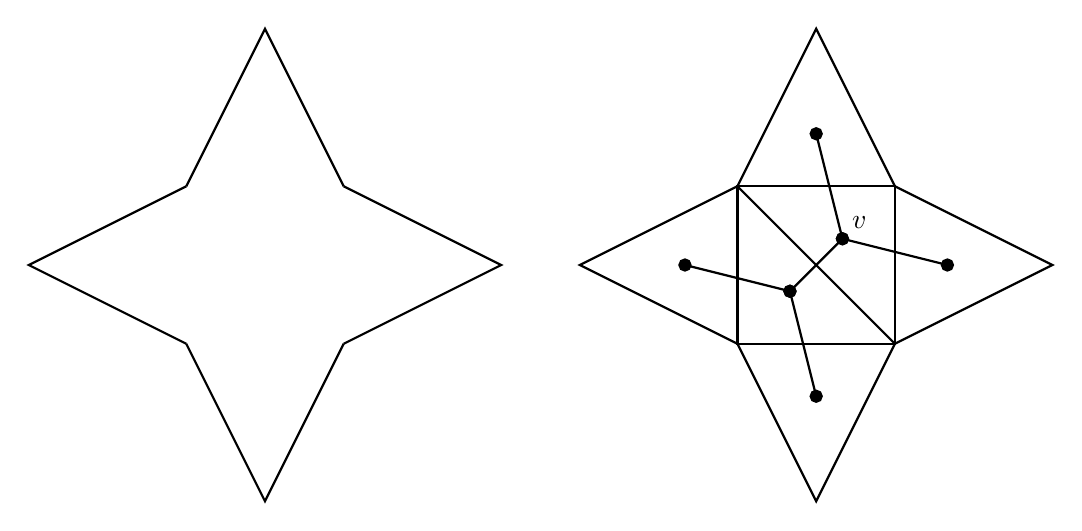
\begin{tikzpicture}[
            boundary/.style={
                thick
            },
            dual/.style={
                thick,
            },
            v/.style={
                insert path={circle[radius=2pt]}
            }
        ]
        \begin{scope}[shift={(-3.5,0)}]
            \draw[boundary] (-1, 1) -- ++( 1, 2) -- ++( 1,-2);
            \draw[boundary] (-1,-1) -- ++( 1,-2) -- ++( 1, 2);
            \draw[boundary] (-1, 1) -- ++(-2,-1) -- ++( 2,-1);
            \draw[boundary] ( 1, 1) -- ++( 2,-1) -- ++(-2,-1);
        \end{scope}
        \begin{scope}[shift={(3.5,0)}]
            \draw[boundary] (-1, 1) rectangle (1,-1);
            \draw[boundary] (-1, 1) -- (1,-1);
            \draw[boundary] (-1, 1) -- ++( 1, 2) -- ++( 1,-2);
            \draw[boundary] (-1,-1) -- ++( 1,-2) -- ++( 1, 2);
            \draw[boundary] (-1, 1) -- ++(-2,-1) -- ++( 2,-1);
            \draw[boundary] ( 1, 1) -- ++( 2,-1) -- ++(-2,-1);

            \newcommand{\trinner}{5/3}
            \filldraw[dual] ({-\trinner}, 0) [v] -- ({-1/3}, {-1/3}) [v];
            \filldraw[dual] (0, {-\trinner}) [v] -- ({-1/3}, {-1/3}) [v];
            \filldraw[dual] ({\trinner}, 0) [v] -- ({1/3}, {1/3}) [v];
            \filldraw[dual] (0, {\trinner}) [v] -- ({1/3}, {1/3}) [v];
            \filldraw[dual] ({1/3}, {1/3}) -- ({-1/3}, {-1/3});
            
            \draw ({1/3},{1/3}) node[anchor=south west] {$v$};
        \end{scope}
        \end{tikzpicture}
    \end{center}
    The marked node $v$ has degree $3$. \hfill\qedsymbol
\end{solution}

\section*{Problem 4}
Give the pseudo-code of the algorithm to compute a 3-coloring of a triangulated simple polygon. The algorithm should run in linear time.

\begin{solution}
    The proof that any triangulation of a simple polygon can be $3$ colored provides the structure on how to algorithmically color it.
    \begin{algorithm}[H]
        \caption{Triangulation 3-Coloring}
        \begin{enumerate}
            \item Construct the dual graph $G$ from the given triangulation
            \item Pick some face $f$ from the triangulation
            \item Color each vertex of $f$ with a different color
            \item Perform a DFS starting at $f$ over $G$
                \begin{itemize}
                    \item Each new face will be adjacent to a colored face, hence two vertices are already colored
                    \item Color the remaining vertex with the only possible color
                \end{itemize}
        \end{enumerate}
    \end{algorithm}
    As for time complexity:
    \begin{enumerate}
        \item Constructing the dual graph takes $O(n)$ time. Alternatively one can employ an existing DCEL to traverse the polygon, but the upper bound in either case for making the representation is $O(n)$.
        \item Picking some face from the triangulation/dual graph can be done in $O(1)$.
        \item The number of nodes in the dual graph is $O(n)$ meaning the DFS traversal is also $O(n)$.
    \end{enumerate}
    Overall then the running time of the algorithm is $O(n)$.
\end{solution}

\section*{Problem 5}
Can the algorithm of this chapter also be used to triangulate a set of $n$ points? If so, explain how to do this efficiently.

\begin{solution}
    The key idea is that we can efficiently find the convex hull of the points and split it into 2 monotone polygons, of which can be triangulated in linear time. The convex hull can be found in $O(n \log n)$ time. Consider then the set of vertices in the convex hull but not on its boundary. These can be sorted such that they are increasing montonically with respect to their $x$-coordinate in $O(n \log n)$ time as well. Therefore the convex hull can be split into monotone halves by connecting these inner vertices where there are edges between adjacent $x$ coordinate vertices. Each half then can be triangulated in $O(n)$ time. Hence in total the set of $n$ point can be triangulated in $O(2 n \log n + 2n) = O(n \log n)$ time.
\end{solution}

\end{document}
